\documentclass[12pt]{beamer}
\usepackage[UKenglish]{babel}% http://ctan.org/pkg/babel
\usepackage[UKenglish]{datetime}
\usepackage[export]{adjustbox}
\usepackage{tikz}
\usepackage{pgfplots}
\usepackage{caption}
\pgfplotsset{compat=1.17}
\usepackage{pgfpages}
\usetheme{Dresden}
\usecolortheme{seahorse}
\usefonttheme{structuresmallcapsserif}
\usefonttheme{serif}
\usepackage[T1]{fontenc}
\beamertemplatenavigationsymbolsempty

\newcommand\blfootnote[1]{%
\begingroup
\renewcommand\thefootnote{}\footnote{#1}%
\addtocounter{footnote}{-1}%
\endgroup
}
% \setbeameroption{show notes on second screen}

\hypersetup{pdfpagemode=FullScreen}
% Class options include: notes, notesonly, handout, trans,
%                        hidesubsections, shadesubsections,
%                        inrow, blue, red, grey, brown

% Theme for beamer presentation.
\usepackage{beamerthemesplit} 
% Other themes include: beamerthemebars, beamerthemelined, 
%                       beamerthemetree, beamerthemetreebars

\title{Dispersion Corrections in Density Functional Theory}    % Enter your title between curly braces
\author{\itshape Samuel  Frost}                 % Enter your name between curly braces
\institute{University of Nottingham}      % Enter your institute name between curly braces
\date{\today}                    % Enter the date or \today between curly braces

\begin{document}
% Creates title page of slide show using above information
\begin{frame}
  \titlepage
\end{frame}
\note{Talk for 10 minutes} % Add notes to yourself that will be displayed when
                           % typeset with the notes or notesonly class options
                           
\begin{frame}
  \frametitle{What is DFT?}
  \begin{itemize}
    \item A computational chemistry method which uses the principles of quantum mechanics to model the electronic structure of a chemical system, thus pulling out many important properties
    \item Uses functionals of the local electron density, more accurate 'GGA' methods which use a 
    \emph{gradient} of the electron density exist e.g. PBE \& BLYP 
  \end{itemize}
\end{frame}

\begin{frame}
  \frametitle{DFT's Successes and Failures}
  \begin{itemize}
    \item<1-> DFT works very well for crystals that are purely ionic or covalent
    \item<2-> DFT cannot accurately model dispersion interactions
    \item<2-> This causes DNA to unravel and graphene sheets to repel each other
  \end{itemize}
\end{frame}

\begin{frame}
  \frametitle{Stefan Grimme to the rescue}
  \begin{itemize}
    \item In 2006 Stefan Grimme introduced DFT-D2, a method of correcting a functional to include dispersion interactions\footnotemark
    \item A more extensive and accurate based off of his previous DFT-D method
    \item This method was so cheap and accurate that it's still used to this day 
  \end{itemize}
  \footnotetext{Semiempirical GGA-type density functional constructed with a long-range dispersion correction, https://doi.org/10.1002/jcc.20495}
\end{frame}

\begin{frame}
  \frametitle{How does DFT-D2 work?}
  \begin{itemize}
    \item Pairwise attraction between distinct atoms $i$ and $j$ for all $N$ atoms, where $R_{i,j}$ is their separation
  \end{itemize}
  $$E_\text{disp} = -s_6 \sum_i^{N-1} \sum_{j=i+1}^{N} \frac{C_6^{i,j}}{R_{i,j}^6}f_\text{damp}(R_{i,j})$$
  \begin{itemize}
    \item $C_6^{i,j} = \sqrt{C_6^iC_6^j}$ is the \emph{dispersion coefficient}
    \item $C_6^i = 0.05NI_i\alpha_i$, where $N$ is a scaling factor depending on its row, $I$ is the first ionisation energy and $\alpha$ is the polarisability
  \end{itemize}
\end{frame}

\begin{frame}
  \frametitle{Fermi Damping Function}
  \begin{center}
    \begin{tikzpicture}
      \begin{axis}[
        width=210pt,
        xlabel = \(R_{i,j}\),
        ylabel = {\(f_\text{damp}(R_{i,j})\)},
        ]
        \addplot[
          color=blue,
          domain=0:2,
          samples=50,
          width=5pt,
          ]
          {1/(1+exp(-10*x+10))};
        \end{axis}
      \end{tikzpicture}
    \end{center}
    $$f_\text{damp}(R_{i,j}) = \frac{1}{1 + \exp(-d(R_{i,j}/R_r) - 1))}$$
\end{frame}

\begin{frame}
  \frametitle{Effectiveness}
  \framesubtitle{Black Phosphorus}
  With the correct functional, DFT-D2 can help predict the exact equilibrium distance between sheets!\footnotemark
  \begin{center}
    \begin{tabular}{ c|c|c|c|c|c } 
      &LDA & LDA-D2 & PBE & PBE-D2 & optB86b-vdW \\ 
      \hline
      $d_0$ / \AA & 2.93 & 2.89 & 3.42 & 3.09 & 3.09
    \end{tabular}
    \end{center}
  \footnotetext{Effect of van der Waals interaction on the structural and cohesive
  properties of black phosphorus}
\end{frame}

\begin{frame}
  \frametitle{Ineffectiveness}
  \framesubtitle{Metals Gasses}
  \begin{itemize}
    \item \small{DFT-D2 overestimates vdW interactions on metal surfaces \footnotemark }
  \end{itemize}
  \begin{figure}
    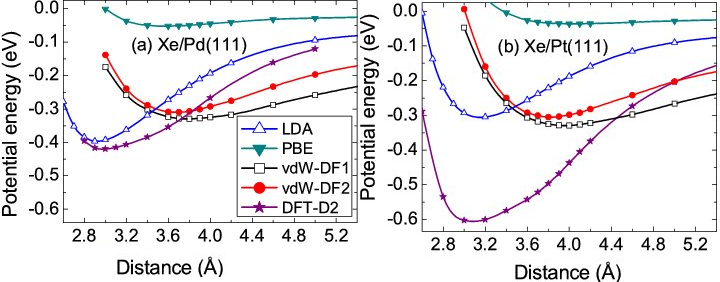
\includegraphics[width=300pt]{chen.jpg}
  \end{figure}
  \footnotetext{{The Role of van der Waals Interactions in the Adsorption of Noble Gases on Metal Surfaces, 10.1088/0953-8984/24/42/424211}}
\end{frame}

\begin{frame}
  \frametitle{Ineffectiveness}
  \framesubtitle{Extreme Conditions}
  \begin{itemize}
    \item Under extreme conditions DFT-D2 can begin to break down, and actually give worse results than no dispersion correction at all\footnotemark
  \end{itemize}
  \captionsetup[figure]{font=tiny}
  \begin{figure}
    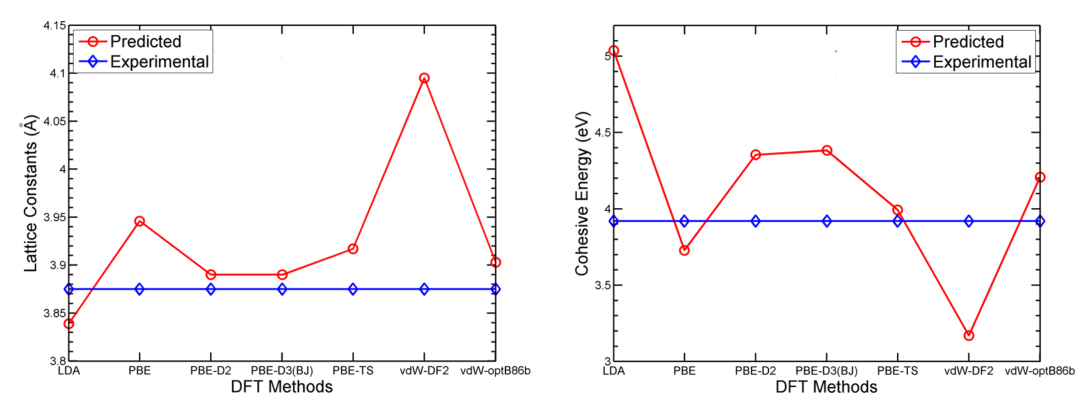
\includegraphics[width=300pt]{palladium.jpg}
    \caption{Shown here is the lattice constant and cohesive energy for Paladium Hydride under extreme stress}
  \end{figure}
  \footnotetext{\tiny{Breaking Badly: DFT-D2 Gives Sizeable Errors for Tensile Strengths in
  Palladium-Hydride Solids}}
\end{frame}

\begin{frame}
  \frametitle{Other Criticisms}
  \begin{itemize}
    \item The aforementioned $s_6$ scaling factor and $d$ in the fermi damping function are both \emph{fit} to emperical data
    \item The $C_6$ constant does not account for the \emph{environment} of the atom, $C_6$ for carbon in methane is the same as $C_6$ for carbon in benzene
  \end{itemize}
\end{frame}

\begin{frame}
  \frametitle{DFT-D3}
  \begin{itemize}
    \item DFT-D3 uses the coordination number of the atom to help account for the chemical environment\footnotemark
    \item Uses higher order terms \emph{e.g.} $C_8$
  \end{itemize}
  \footnotetext{Density functional theory with London dispersion corrections, 10.1002/wcms.30}
\end{frame}

\begin{frame}
  \frametitle{Non-local Density Dependent Corrections}
  \begin{itemize}
    \item Only depend on the electron density at two coordinates, DFT functionals normally depend on a single location in space\footnotemark
    \item Derived entirely from first principles, in contrast to DFT-D2/3 which depend on many experimental values and even requires fitting parameters
    \item Incredibly expensive to run, can take months to run even on expensive hardware, in contrast to DFT-D2 which can easily run on your laptop
  \end{itemize}
  \footnotetext{Dispersion-Corrected Mean-Field Electronic Structure Methods}
\end{frame}

\begin{frame}
  \frametitle{Conclusion}
  \begin{itemize}
    \item For fast results under normal conditions, DFT-D2/3 or any other semi-emperical method is ideal, especially for those on a budget
    \item For accurate results and edge cases, non-local density dependent corrections may be favourable
  \end{itemize}
\end{frame}

\begin{frame}
  \frametitle{\emph{The End}}
  \centering{\LARGE{\emph{Fin.}}}
\end{frame}

% \begin{frame}
%   \frametitle{References}
%   \begin{thebibliography}{2}

%     \bibitem{rod}
%     https://courses.lumenlearning.com/boundless-physics/chapter/elasticity-stress-strain-and-fracture/

%     \bibitem{youngs}
%     John Martin

%   \end{thebibliography}

% \end{frame}

\end{document}
